\documentclass{acm_proc_article-sp}
\usepackage{url}
\usepackage{listings}
\raggedbottom

%% Bring items closer together in list environments
% Prevent infinite loops
\let\Itemize =\itemize
\let\Enumerate =\enumerate
\let\Description =\description
% Zero the vertical spacing parameters
\def\Nospacing{\itemsep=0pt\topsep=0pt\partopsep=0pt\parskip=0pt\parsep=0pt}
% Redefine the environments in terms of the original values
\renewenvironment{itemize}{\Itemize\Nospacing}{\endlist}
\renewenvironment{enumerate}{\Enumerate\Nospacing}{\endlist}
\renewenvironment{description}{\Description\Nospacing}{\endlist}

% Disable the copyright and boilerplate for now
\makeatletter
\let\@copyrightspace\relax
\makeatother

\begin{document}
\lstset{
	language=Java,
	numbers=left,
	tabsize=2,
	showstringspaces=false,
	basicstyle=\ttfamily\small
}
\conferenceinfo{UWCSE503}{'10 Seattle, WA USA}

\title{JavaGrok: Automatic Inference of Documentation for Under-documented Code}

\numberofauthors{1} 
\author{
\alignauthor
Colin S. Gordon, Reto Conconi, Gilbert Bernstein, Michael Bayne\\
       \affaddr{University of Washington}\\
       \affaddr{Seattle, WA USA}\\
       \email{\{csgordon,conconir,gilbo,mdb\}@cs.washington.edu}
}

\maketitle
\begin{abstract}
Software development increasingly involves the use of third party
libraries. Developers routinely learn the APIs of myriad
libraries in the course of a single software development project. This process
is made more difficult by the fact that many libraries are poorly documented.
The developer often has to read the library source code or resort to trial and
error to determine how to correctly use the library. These methods of learning
about the library are time consuming and error prone.

We present a method to automatically augment library API documentation with
properties inferred by a variety of static analyses. These include argument
nullability, reference leaking and capturing, and conditions that will cause exceptions
to be thrown.
We also perform a user study to
evaluate the usefulness of the additional documentation for developers and
conclude that the area deserves further study.
\end{abstract}

% These categories are from the ACM CCS (Computing Classification System)
% http://portal.acm.org/ccs.cfm
\category{F.3.1}{Specifying and Verifying and Reasoning about
Programs}{Specification techniques}
\category{D.2.7}{Distribution, Maintenance, and Enhancement}{Documentation}
\category{D.2.13}{Software Engineering}{Reusable Software}

% These "terms" are from the ACM's official General Terms classifications.
% http://www.acm.org/about/class/1998
\terms{Documentation, Human Factors, Languages}

\keywords{Documentation Inference, Software Documentation, Static Analysis}

\section{Introduction}

Despite their best intentions, many developers routinely fail to provide
adequate or any documentation for the code they write.  Whether because of poor
practice, lack of time or a sincere belief on the part of programmers that their
code will soon be thrown away, much code in regular use remains undocumented.
New developers join the team, the code is handed off to another group, or
perhaps even posted publicly on the Internet.  By various means, this code
finds its way into the hands of programmers who---having been assured that this
code will save them weeks of effort---now face a thoroughly unenviable task:
grok a lump of un(der)documented code and learn its interface well enough
to solve their original problem.

We believe it would be useful to have a tool that could generate partial
documentation of at least simple properties.

The prototype tool we describe here, JavaGrok, seeks to do just this.  By
applying static analyses to infer properties of library source code and then
translating the results into human readable form, we are able to
automatically construct or augment Javadoc documentation.
Using this tool, we
consider the hypothesis that a significant amount of user pain and frustration
with un(der)documented libraries is due to confusion about
properties discoverable via static analyses. We consider analyses for argument nullability,
reference leaking and capturing, and exceptional conditions.
Here, we focus on confusions about formal properties
rather than conceptual
or higher level confusions about the proper way to use a library.

Although there has been previous work on automatic
documentation~\cite{autodoc}, we perform the first user study
focused on whether automatically generated documentation is helpful for program
understanding.  By contrast, previous work~\cite{autodoc, Nimmer2002} has
evaluated the benefit of program analyses to users in verification tasks or the
accuracy of generated annotations relative to exemplar documentation.
We believe that determining whether automatically generated documentation helps
developers understand code is the logical next step, and more relevant to practice.

Our user study compares developers'
experience using a poorly documented library with and without JavaGrok
annotations.  We measured how often users were confused and how they resolved their confusion.  We also collected qualitative exit
questionnaires.  Unfortunately, we found no evidence that JavaGrok had
significant impact, positive or negative on the user experience.  We discuss
reasons why our evaluation was not conclusive and possible alternative
evaluations later.


\section{Example}
\label{sec:Example}

Consider Figure \ref{fig:pre}, a na\"ive collection object.
A programmer looking at the method interface of 
\texttt{public Object getAll()} does not know
that \texttt{getAll()} will leak a reference to its
internal representation. This might be surprising
if the list of objects that gets returned keeps growing
even though the caller of \texttt{getAll()} does not add those objects.

\begin{figure}[t]
\begin{lstlisting}
public class A
{
	private LinkedList<Object> list;
		
	public A() {
		list = new LinkedList<Object>();
	}
		
  public void add(Object o) {
   	list.add(o);
  }
    
	public List<Object> getAll() {
		return list;
  }
}
\end{lstlisting}
\caption{An example unannotated class.}
\label{fig:pre}
\end{figure}

But with information about reference leaks and captures added, a programmer can 
determine that she or he will not have an unique reference
to the list of all objects.  Knowing the reference is still shared by the
library, a developer may decide to copy the content 
of the list into a newly created list.  Figure \ref{fig:postannotation}
shows a class annotated with reference leak and capture information produced by
our tool.

\begin{figure}[t!]
\begin{lstlisting}
public class A
{
	private LinkedList<Object> list;
	
	@UniqueReturn
	public A() {
		list = new LinkedList<Object>();
	}
		
  public void add(@Retained Object o) {
   	list.add(o);
  }
  
	@NonUniqueReturn
	public List<Object> getAll() {
		return list;
  }
}
\end{lstlisting}
\caption{An example class annotated with capture and leak information.}
\label{fig:postannotation}
\end{figure}

For a simple example such as this, inspecting the library code is not a
significant burden for the developer.  But as library size and complexity grow,
it is preferable to refer to condensed documentation rather than
deciphering library code.
Fortunately Javadoc will reproduce any source annotations in the HTML
documentation it produces.  For \texttt{getAll()}, the documentation will
include the annotations JavaGrok added.


\begin{figure*}
\centering
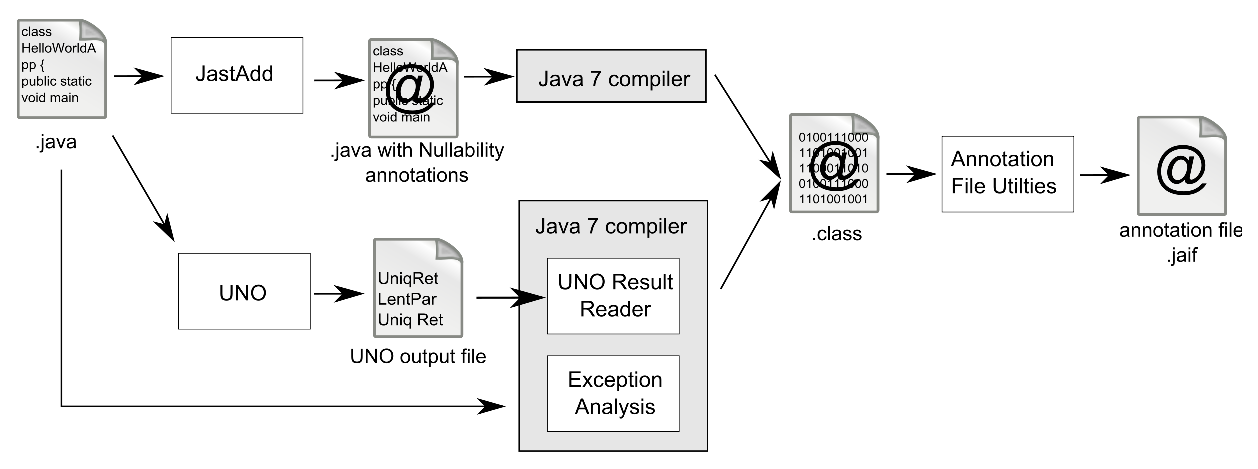
\psfig{file=figures/technicalApproach/from_source_to_jaif.eps, width=5.0in}
\caption{JavaGrok's toolchain from source to JAIF}
\label{fig:from_source_to_jaif}
\end{figure*}

\section{Analyses}

In this section we describe the analyses we perform: their implementation,
output, and why each analysis would be useful for a developer.

\subsection{Javarifier}
\label{sec:Javarifier}

Javarifier is a tool to infer reference immutability information built in
conjuction with research done by Quinonez et al.~\cite{Javarifier}. It infers
mutability constraints for object fields, method arguments and receivers.  We
use \textit{mutate} to mean updating the value of an object's fields, calling a
method on an object that updates the values of its fields, or calling a method
on an object that mutates an object referenced by one of its fields.

Below we enumerate the annotations inferred by Javarifier which are utilized by
JavaGrok, and a summary of what they communicate to the developer:

\texttt{@ReadOnly} When appearing on a method, this indicates to the developer
that the method will not mutate its receiver. When appearing on a method
argument, this indicates to the developer that the method will not mutate the
argument through the supplied reference.

\texttt{@Mutable} When appearing on a method, this indicates to the developer
that the method may mutate its receiver. When appearing on a method argument,
this indicates to the developer that the method may mutate the argument through
the supplied reference.

Javarifier generates two additional annotations which are important for type
checking, but not important when simply communicating method behavior to a
developer.

\texttt{@QReadOnly} appears on type parameters of method arguments, for example
\texttt{List<@QReadOnly Date>}. Such an annotation on a method argument
indicates that the method accepts both \texttt{List<@ReadOnly Date>} and
\texttt{List<@Mutable Date>}. However, the method itself is restricted to only
operations allowed on both read-only and mutable dates, which is strictly a
subset of the operations allowed on read-only dates.

\texttt{@PolyRead} indicates that a method and/or its arguments are polymorphic
over mutability. Such a method may legally be instantiated with
\texttt{@ReadOnly} receiver and/or arguments and thus must not mutate the
receiver or arguments.

We convert both of the above annotations to \texttt{@ReadOnly}, as
that is sufficient to communicate the method's behavior to the developer and we
are not concerned with type-checking mutability.

\subsection{Uno}

Uno infers alias and encapsulation properties.  The
tool generates annotations which provide information about how a certain
function treats its parameters, return values and fields when called. More
concretely, it infers whether or not a function captures or leaks a
reference, or returns a new unique reference.

The tool generates annotations which are stored in a single separate file. 
To integrate the analysis results of UNO into the Java documentation we
use our own framework. We implemented an AST traversal inside the Java 7 
compiler that, at initialization, reads in the file generated by UNO and 
stores the information in a hashset. During the iteration over the AST
our visitor inserts annotation at the appropriate places.

\subsection{Thrown Exceptions}

Java requires that checked exceptions be declared by methods that raise them,
but frequently the conditions under which exceptions are raised are unclear to a
library user. Even with checked exceptions, often a supertype of a thrown
exception is declared.  While knowing that an \texttt{IOException} might be
thrown is useful, knowing that the method might throw either a
\texttt{FileNotFoundException} or \texttt{InterruptedByTimeoutException} is more
useful to a developer, because knowing the specific exception may help to debug
a program; knowing that a \texttt{FileNotFoundException} was thrown tells a
developer to check that file paths are correct and that any tasks that should
have created the file ran correctly, while an \texttt{IOException} could
indicate a variety of problems with local files, or any of a number of problems
with the network.  Additionally, unchecked exceptions need not be declared in Java method
signatures or documentation and can remain entirely invisible to the library
user until they are encountered at runtime.

To alleviate this, we infer some of the conditions under which a method would
throw an exception, and produce annotations of the form:

\begin{verbatim}
@Throws(when =
    "IllegalArgumentException when (x < 0)")
public Object getElement(int x) { ... }
\end{verbatim}

This inferred information can inform developers of unchecked exceptions,
and alert them to otherwise undocumented assumptions of a library without
requiring developers to dig through the library's code.
Annotations may contain a list of exceptions and conditions, and for some
complex conditions we reduce the condition to ``sometimes'' because our analysis
performs no symbolic execution, and is only based on syntactic structure.  We do not use an
existing analysis tool because none were available for this task, but our
simple analysis provides useful results.

\subsubsection{Implementation}

Our exception analysis is implemented in two phases as plugins to the JDK 7 compiler.
In the first phase, the
abstract syntax tree for every method of the program is traversed in the
following manner.  The analysis walks over every statement of the method,
descending recursively into control flow constructs.  The analysis keeps a stack
of conditional branches, pushing branch conditions when entering the positive
branch of a conditional, and negating the most recent condition when entering
the \texttt{else} clause.  A counter is also kept for how many times the
analysis has entered a more complex control structure, such as a loop or
\texttt{switch} statement whose conditions for execution are more complicated,
and require reasoning about iteration and ``falling through'' cases.  When
analysis of a control structure is complete, a clause is popped from the
branch stack or the counter is decremented as appropriate.

When entering a method or a try/catch construct, we push a new empty set of exceptions onto
a stack that tracks what exceptions are thrown at the current level of
\texttt{try} nesting --- the try-stack.
When a throw statement is found, the statement's AST node is added to the
topmost set on the try-stack, 
along with the current branch condition if no complex control structures have
been encountered, otherwise it is added with a flag that the condition was more
complicated than we trace.  When a \texttt{try} body has been traversed, we
remove exceptions from that top set that are subclasses of caught exception
types in the associated \texttt{catch} bodies.  We then merge the topmost set
into the next set on the try-stack, and process the bodies of
the \texttt{catch} clauses.  When traversal of a method is complete, we add the
single remaining set on the try-stack to a hash map from method definition AST
nodes to sets of exception-condition pairs.

{\LARGE TODO: Compare this to the code! I think that actually, we add throws to
the current set \emph{as we filter}, then merge the set, so a throw in a catch
body could potentially be filtered out by a subsequent catch associated with the
same try, which is wrong.}

Method calls are handled in a similar manner, as they are potential sources of
exceptions.  A separate try-stack exists for method calls.  When a call is
encountered, it is added to the set with its condition as for throws, but the
container also has a list of exception types filtered by catch clauses.  When
initially added to the top of the method try-stack, the list is empty.  When
processing the catch clauses associated with a \texttt{try}, the list of each
method call instance in the topmost set of the method try-stack is populated. 

In the second phase, the tree is traversed again, and the mappings from the first
phase is used.  When visiting a method definition, any explicit throws from
methods the current node calls are filtered based on the list of catch clauses
enclosing the calls.  Those throws are then added to the set of uncaught
exceptions from the current method, and the whole group along with their
conditions (either complex, via a method call, or the simple condition under
which the exception is thrown) are serialized and added to that method as an
annotation.  When serializing the conditions for explicit throws of a method
call, any formal parameters of the current method used as actual parameters to
callees replace the corresponding callee formals in the serialized condition.
These annotations are compiled into bytecode, and extracted in a later phase of
JavaGrok.

\subsubsection{Precision}
{\LARGE: Discuss precision.  One-level propagation of only explicit throws,
"check-param" methods, funkiness with throws in catch clauses.}

Buse and Weimer infer documentation for exception conditions
using an analysis that performs full symbolic execution along paths to reach throw
statements, propagating information between methods as necessary~\cite{autodoc}.
Because they
perform full symbolic execution, their tool can be much more precise than ours.
Replacing our exception analysis with theirs, or implementing our own symbolic
execution would likely improve the quality of our exception documentation.  

As in Buse and Weimer's work, we expose internal field names and
local variable names in exceptional conditions.  We agree with their assessment
that while this leaks some
implementation information and is not necessarily informative, in practice
leaked variables are often still useful: for example, showing that an exception is
thrown from a list's \texttt{remove()} method when a local variable \texttt{len}
is equal to 0 has clear implications.

\subsection{Nullability}
\label{sec:Nullability}

In heavily object oriented languages like Java, every variable is nullable,
capable of holding either a reference or the
special value null.  Because of this ubiquity, one common mistake is to call
methods with null parameters they are unprepared to handle, or to erroneously
assume that returned values are never null.  Well documented libraries, like
the Java collections framework, frequently spell out when variables are
assumed to be nullable or not-null, while many libraries with weaker
documentation omit this information entirely.

By means of a nullability type inference~\cite{NonNullTypeInference} we can add
similarly useful information to documentation.  Although the JastAdd analysis
we've chosen to use does not require a whole program, it does make a closed
world assumption; that is, it assumes it is analyzing all code that will ever be
linked with the library.  This leads to optimistic annotation inferences when run on
library code.  JastAdd produces \texttt{@NonNull} annotations, indicating that the user should assume that an
argument or method return value will not assume the value \texttt{null}.


\section{Technical Approach}
To infer information about Java code we use existing Java inference tools and 
combine their output. Additionally we have our own framework which allows us to
implement our own analysis. 

Most inference tools available put annotations into 
the Java class files. So does our own framework. To get the inferred information
back into the source files we use the annotation file utilities \cite{AFU} 
(TODO: How to cite a website???). 
These consist of several tools. One allows to extract annotations
from the class files. Thereby the information gets stored in an external file.
Javarifier - one of the tools which we use - directly supports to generate those
external annotation files. In a next step we use another annotation file utility which
merges the source files with the corresponding annotation files.

\begin{figure}
\centering
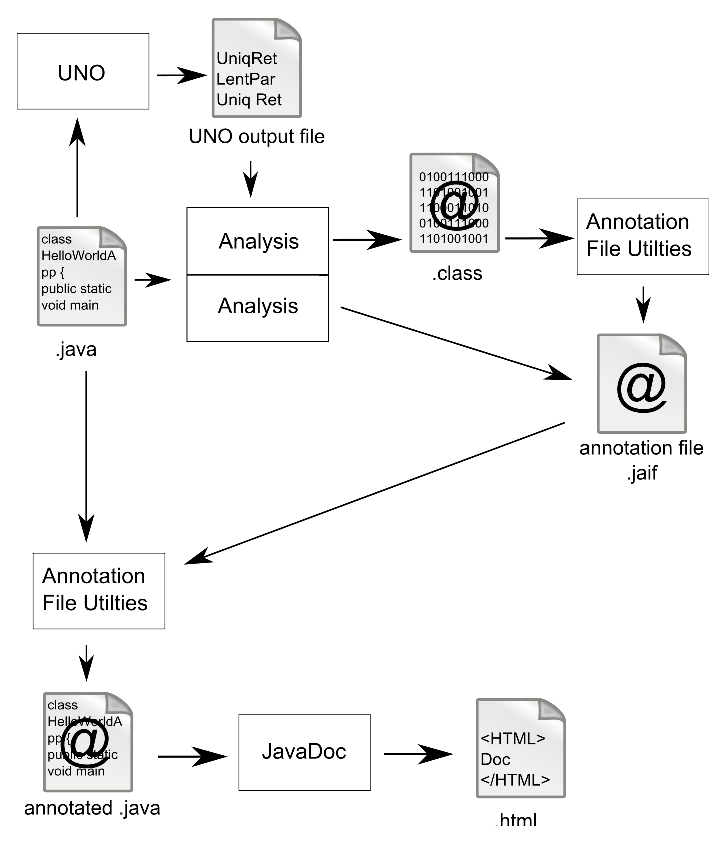
\psfig{file=figures/technicalApproach/technicalApproach.eps, width=2.1in}
\caption{Toolchain}
\end{figure}

\subsection{Analysis Framework}

To implement our own analysis tools we use the current version of the Java 7 compiler.
This allows us to use it's plugin architecture to write our own analyzers. From within
a Java compiler plugin we can access the compiler's abstract syntax tree and we can emit 
annotation to the class files. As described above those annotation will get extracted 
with the annotation file utilities.


\section{Evaluation} \label{sec:Evaluation}
We performed a small experiment wherein developers were given a third party
library with documentation and a set of programming tasks. They were asked to report on certain
events that occurred while completing the tasks. We specifically focused on
when the developer had questions about how to correctly use the library, and
considered four cases: a) the question was answered by our annotations, b) the
question was answered by the existing library documentation, c) the question
was answered by reading the library source code, and d) the question was not
answered. We also asked the developers to note any time they were surprised by
the library's behavior.

Our hypothesis was that by augmenting library documentation with inferred
properties, we would decrease the frequency with which developers needed to
refer to the library source code to answer questions. This would show up as a
non-zero incidence of questions being answered by annotations and a
corresponding decrease in the questions that were answered by reading source
code. We also hypothesized that our annotations may have resulted in a
reduction in surprise at library behavior, and would not increase the incidence
of surprise.

\begin{figure*}
\centering
\begin{tabular}{ l | r r r r | r }
 & \multicolumn{4}{| c | }{Question answered by:} & \\
Developer & Annotations & Docs & Source & Unanswered & Surprised \\
\hline
Dev 1 & 0 & 14 & 0 & 1 & 0 \\
Dev 2 & 1 &  5 & 2 & 1 & 0 \\
Dev 3 & 1 &  3 & 0 & 0 & 0 \\
Dev 4 & 1 &  6 & 1 & 1 & 0 \\
\hline
\textit{Experiment} & 3 & 28 & 3 & 3 & 0 \\
\hline
Dev 5 & - &  4 & 0 & 0 & 0 \\
Dev 6 & - & 13 & 2 & 3 & 1 \\
Dev 7 & - & 10 & 0 & 2 & 0 \\
Dev 8 & - &  7 & 1 & 2 & 1 \\
\hline
\textit{Control} & - & 34 & 3 & 7 & 2 \\
\hline
\end{tabular}
\caption{Experiment Results}
\label{fig:exp_results}
\end{figure*}

\medskip
\subsection{Experiment Design}
The experiment involved two groups of four developers each, all of whom were
University of Washington computer science graduate students. The developers
were given a set of programming tasks involving the creation of simple
interactive animations. They were supplied with the Nenya~\cite{nenya} graphics
and animation library to use to complete those tasks. None of the developers had
previously seen or used the library. The experimental group was provided with
augmented documentation and source code for the library, and the control group
was provided with original, unmodified documentation and source code.

There were four tasks that were designed to consume at least one
hour. Developers were told that they were free to leave after one hour, even if
they had not completed all of the tasks.

The members of each group were provided with the Eclipse IDE, configured to
provide ready access to the appropriate documentation and source code. As the
subjects' experience with the Eclipse IDE was quite varied, they were shown how
to access both the library documentation and source code. The aim was to reduce
the likelihood that differing familiarity with the IDE would influence their
decision to inspect the documentation or source.

The subjects were instructed to first check the documentation when they
encountered a question about correct usage of the library, then to consult the
source code only if their question was not answered to their satisfaction by
the documentation. Finally they were asked to record the outcome of each event.
The experimenter could record a question as being resolved by ``annotations'',
``documentation'', ``source code'' and ``not resolved''. The control group had
only the latter three choices as they had unaugmented documentation.

We also instructed subjects to complete a short survey after finishing the
experimental tasks. The results of this survey were not intended to directly
validate or refute our hypothesis, but to help us to gauge other aspects of the
work, better understand ambiguous results, and to direct future work. Data from
the survey are mentioned in the discussion below. The results of our experiment
are shown in Figure ~\ref{fig:exp_results}.

\subsection{Discussion}
For our small test group, a striking difference between the control and
experimental groups would have been necessary to support our hypothesis.  The
results had no such strong
trends, rather they were inconclusive.  Our sample size of developers was not
large enough to be statistically significant, but the developer surveys exhibit
a mixture of both positive and negative trends.

Most developer complaints from both the experimental and control groups were
about the high-level usage model of the library being unclear.  This suggests
the evaluation task was
a poor choice for evaluating our tool; our tool infers small technical
properties of the code, not use models for the library.  A better task would
have required use of our annotations or close source inspection to avoid some
subtle bugs.  Only the control group ever said they were surprised by library
behavior, but the surprises were about higher-level component interactions such
as what order to call a pair of methods, not about properties JavaGrok can
infer.

None of the developers in the experimental group found the annotations to be
frequently useful.  None answered more than one question using the
annotations, which was never more than 1/9th of a subject's questions.  Most
questions for both groups were answered by reading the existing documentation.

There was however some positive feedback from the experimental group.  All
found the annotations to be of a useful level of detail, and 3 of 4 said they
considered the annotations
to be potentially useful, but not for the evaluation task.  This generally
positive response reinforces our belief that the properties
JavaGrok infers could be useful.  It is also possible that other properties
exist that could have been inferred and would have been useful for our chosen
evaluation task.

In designing
our experimental task, we struggled to find a balance between designing a
realistic task, and designing a task geared towards requiring annotations.  We
settled on a task we felt was reasonably general and might benefit from the
generated annotations.  Designing a task specifically to make the annotations useful would
not have helped us understand how useful they were generally, but the situations
where they would provide benefit seem not appear to occur in such a short exercise.
Upon reflection, we suspect that the target experiment time of one hour per
subject, chosen to encourage volunteers, may simply not be enough time to run
into tricky cases where the very particular information JavaGrok documents would
be useful.  We suspect that the annotations might prove valuable in a longer
study, using a library over a longer period of time, allowing more time to run
into what we acknowledge are usually corner cases where specific information
about JavaGrok's properties would prove useful.  One of our subjects said he
suspects they may prove more useful in debugging than in development.

While our actual results showed no significant benefit to JavaGrok's annotations
for this task, the generally positive response to the idea from our test
subjects suggests that automatically inferred documentation deserves more
thorough study.



\section{Related Work}
There is a wealth of work on inferring interesting properties of existing code,
but most of these are focused on inferring properties suitable for checking.
Because our goal is not to prove absence of errors, but to simply infer correct
information that is useful to the developer, some flexibility is available to us
that is not possible for much of that work.

The most directly relevant work is Buse and Weimer's system for automatically
inferring documentation for conditions that will result in a Java method
throwing an exception \cite{autodoc}.  We use a modification of their
algorithm, and also perform several other analyses to provide a broader range
of information.

\subsection{Individual Analyses}
Some text for nullability.

Some text for mutability.

Some text for reference capture and leakage.

Buse and Weimer \cite{autodoc} automatically infer documentation for
exceptions, and the exception analysis in our work is directly based on the
refined version of {\sc Jex} [citation needed] they present.


% \section{Conclusion}

\section{Division of Labor}

Michael is developing the basic toolchain, integrating the mutability analysis
and documenting the evaluation process. Colin set up the \LaTeX~report
structure, is integrating the exception documentation analysis and documenting
the broader related work. Reto is integrating the leaking and capturing
analysis and documenting the main technical approach. Gilbert is integrating
the nullability analysis and handling introductions and conclusions. If
existing tools for exception documentation, leaking and capturing, and
nullability cannot be obtained or usefully integrated, the respective parties
may reimplement the analyses using a simple framework Michael developed using
\texttt{javac}'s plugin API.  The evaluation itself, both the exemplar
comparison and the user study will be load balanced as evenly as possible across
all members, depending on scheduling issues.


%ACKNOWLEDGMENTS are optional
\section{Acknowledgments}
The authors are grateful for the assistance of their volunteer user study
subjects.

\bibliographystyle{abbrv}
\bibliography{javagrok}

\end{document}
